\newpage
\subsection{Feature selection}
Nella terza fase ci siamo focalizzati sulla feature selection con l’obiettivo di definire delle caratteristiche, anche chiamate feature, metriche, o variabili indipendenti che possano caratterizzare gli aspetti principali del nostro problema in esame e, quindi, avere una buona potenza predittiva. Abbiamo utilizzato un metodo della libreria \textit{matplotlib}, il quale ci ha permesso di visualizzare le dipendenze tra le diverse variabili.

\begin{figure}[h]
    \centering
    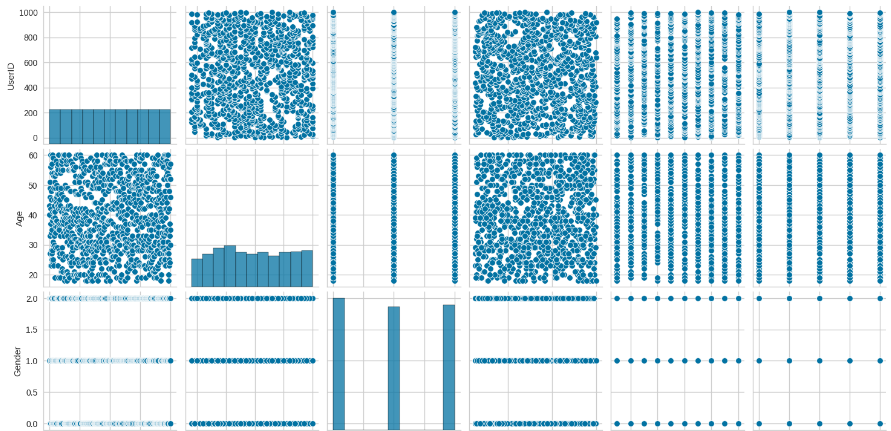
\includegraphics[width=\textwidth]{MetaClassAI_Documentazione/3/img/FeatureSelection_1.png}
\end{figure}
\begin{figure}[h]
    \centering
    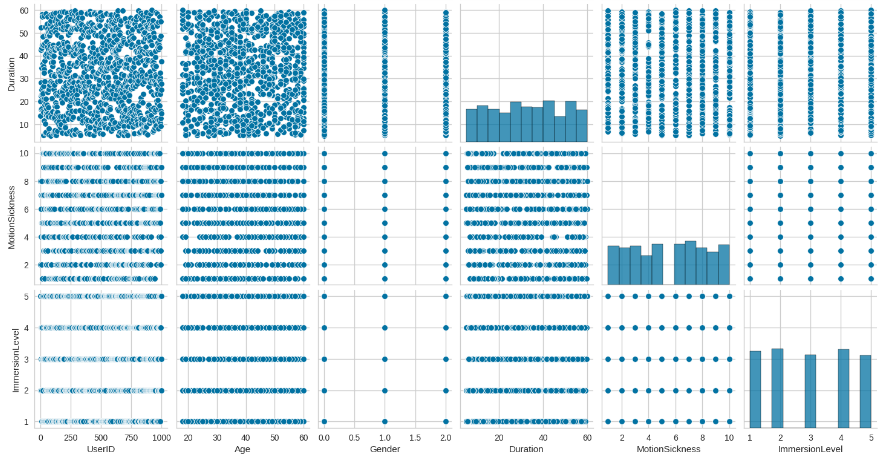
\includegraphics[width=\textwidth]{MetaClassAI_Documentazione/3/img/FeatureSelection_2.png}
\end{figure}